\documentclass[12pt]{book}
\usepackage{amssymb}
\usepackage{amsmath}
\usepackage{amsthm}
\usepackage{amsfonts}
\usepackage{mdframed}
\usepackage{tikz-cd}
\usepackage{stmaryrd}
\usepackage{hyperref}
\setlength{\evensidemargin}{0.25in}
\setlength{\oddsidemargin}{0.25in}
\setlength{\textwidth}{6in}
% \parskip0.2em
\usepackage[utf8]{inputenc}

\DeclareFontFamily{U}{min}{}

\DeclareFontShape{U}{min}{m}{n}{<-> udmj30}{}

\newcommand\yo{\!\text{\usefont{U}{min}{m}{n}\symbol{'207}}\!}

\newmdtheoremenv{theorem}{Theorem}[section]
\newmdtheoremenv{lemma}[theorem]{Lemma}
\newmdtheoremenv{proposition}[theorem]{Proposition}
\newmdtheoremenv{corollary}[theorem]{Corollary}
\newmdtheoremenv{conjecture}[theorem]{Conjecture}
\theoremstyle{remark}
\newtheorem{assumption}[theorem]{Assumption}
\newtheorem{property}[theorem]{Property}
\newmdtheoremenv{remark}[theorem]{Remark}
\theoremstyle{definition}
\newmdtheoremenv{definition}[theorem]{Definition}
\newtheorem{example}[theorem]{Example}
\newtheorem{exercise}{Exercise}[section]
\numberwithin{equation}{section}
\allowdisplaybreaks[1]

%Peng's command
\newcommand{\MW}{Milnor-Witt\ }
\newcommand{\rMW}{\mathrm{MW}}
\newcommand{\KMW}{\mathrm{K}^\mathrm{MW}}
\newcommand{\KM}{\mathrm{K}^\mathrm{M}}
\newcommand{\sKMW}{\mathscr{K}^\mathrm{MW}}
\newcommand{\tbb}[1]{\widetilde{\mathbb{#1}}}
\newcommand{\wt}[1]{\widetilde{#1}}
\newcommand{\af}{\mathbb{A}}
\newcommand{\afnz}[1]{\mathbb{A}^{#1}\setminus \{0\}}
\newcommand{\nonZero}{\setminus \{0\}}
\newcommand{\cO}{\mathcal{O}}
\newcommand{\cC}{\mathcal{C}}
\newcommand{\cD}{\mathcal{D}}
\newcommand{\cX}{\mathcal{X}}
\newcommand{\cY}{\mathcal{Y}}
\newcommand{\cF}{\mathcal{F}}
\newcommand{\cG}{\mathcal{G}}
\newcommand{\bR}{\mathbb{R}}
\newcommand{\bC}{\mathbb{C}}
\newcommand{\bZ}{\mathbb{Z}}
\newcommand{\bfZ}{\mathbf{Z}}
\newcommand{\tbZ}{\tbb{Z}}
\newcommand{\inv}{^{-1}}%
\newcommand{\Gm}{\mathbb{G}_m}
\newcommand{\tGm}{\tbb{G}_m}
\newcommand{\Sp}{\mathrm{Sp}}
\newcommand{\GL}{\mathrm{GL}}
\newcommand{\SL}{\mathrm{SL}}
\newcommand{\MSp}{\mathrm{MSp}}
\newcommand{\BSp}{\mathrm{BSp}}
\newcommand{\SH}{\mathcal{SH}}
\newcommand{\Da}{D_{\af^1}}
\newcommand{\Daba}[1]{D(Ab_{\af^1}(#1))}
\newcommand{\DM}{\mathrm{DM}}
\newcommand{\DMt}{\widetilde{\mathrm{DM}}}
\newcommand{\M}{\mathrm{M}}
\newcommand{\Mt}{\wt{\mathrm{M}}}
\newcommand{\Meta}{\wt{\mathrm{M}}_{\eta}}
\newcommand{\HH}{\mathrm{H}_{\rMW}}
\newcommand{\Heta}{\mathrm{H}_{\eta}}
\newcommand{\sBra}[1]{\left[#1\right]}
\newcommand{\aBra}[1]{\left<#1\right>}
\newcommand{\llBra}[1]{\llbracket #1 \rrbracket
}
\newcommand{\Set}{\mathbf{Set}}
\newcommand{\Top}{\mathbf{Top}}
\newcommand{\Ring}{\mathbf{Ring}}
\newcommand{\Cart}{\mathbf{Cart}}
\newcommand{\Hom}{\mathrm{Hom}}
\newcommand{\Map}{\mathrm{Map}}
\newcommand{\Ker}{\mathrm{Ker}}
\newcommand{\Fun}{\mathrm{Fun}}
\newcommand{\PSh}{\mathrm{PSh}}
\newcommand{\Sh}{\mathrm{Sh}}
\newcommand{\Op}{\mathrm{Op}}
\newcommand{\op}{\mathrm{op}}
\DeclareMathOperator{\Spec}{\mathrm{Spec}}
\newcommand{\Spc}{\mathcal{S}pc}
\DeclareMathOperator*{\Lim}{\mathrm{Lim}}
\DeclareMathOperator*{\Colim}{\mathrm{Colim}}
\newcommand{\xr}[1]{\xrightarrow{#1}}

\newcommand{\AZ}{\mathbb{A}\mathcal{Z}}
\newcommand{\bfZa}{\mathbf{Z}_{\mathbb{A}^1}}

\raggedbottom

\title{Seeing the Mountain}
\author{Keyao Peng}



\begin{document}
\begin{titlepage}
\begin{center}
{\huge\bfseries Seeing the Mountain \\}
% {\Large A Journey Through Post-Modern Geometry \\}
 % ----------------------------------------------------------------
 \vspace{1.5cm}
 {\Large\bfseries Keyao Peng}\\[5pt]
 keyao.peng@ube.fr\\[14pt]
  % ----------------------------------------------------------------
 \vspace{2cm}
 % ----------------------------------------------------------------
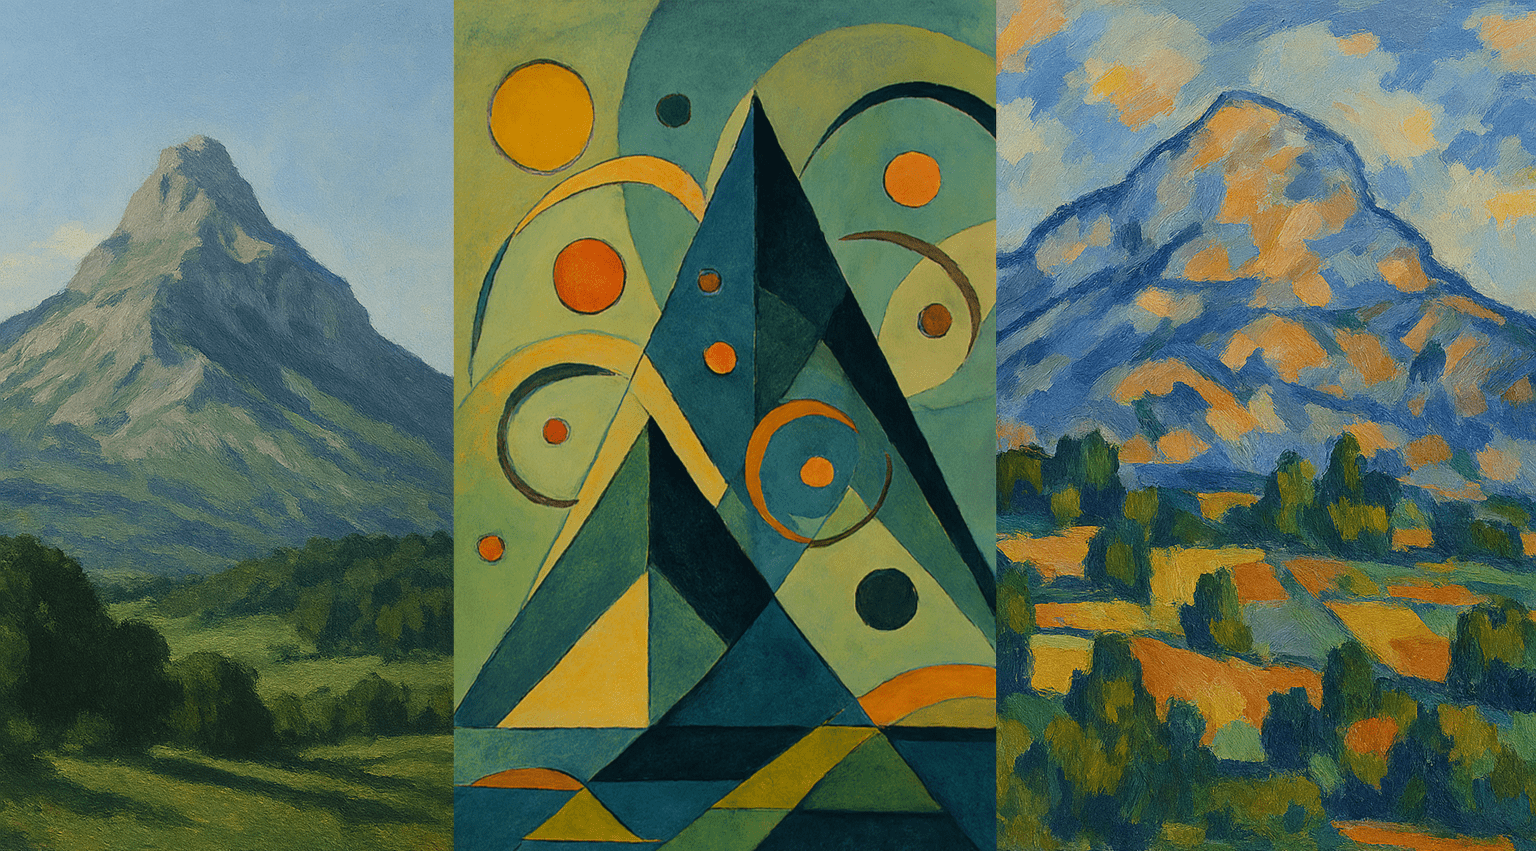
\includegraphics[width=\textwidth]{cover.png}\\[5pt]
 \vfill
{Sep 2025}
\end{center}
\end{titlepage}

{\clearpage

\thispagestyle{empty}
\newlength{\longest}
\settowidth\longest{\huge\itshape Seeing the mountain still as a mountain.}
\null\vfill

\centering
\parbox{\longest}{%
  \raggedright{\huge\itshape%
  Seeing the mountain as the mountain; \\ 
  Seeing the mountain as not a mountain; \\ 
  Seeing the mountain as still a mountain. \par\bigskip
  }   
  \raggedleft\Large\MakeUppercase{Qingyuan Xingsi}\par%
}

\vfill\vfill

\clearpage}

\tableofcontents
\setcounter{chapter}{-1}
\chapter{Introduction}\label{chap:introduction}


\section{What is Algebraic Geometry?}

Algebraic geometry is the study of geometric spaces that locally arise as solutions to polynomial equations. This study can be approached at two levels:

\begin{itemize}
  \item \textbf{Local:} This involves studying the geometric properties of solution sets to polynomial equations. Since we work not only over $\mathbb{R}$ or $\mathbb{C}$ but potentially over arbitrary fields or rings, we must construct a more intrinsic notion of geometry associated with algebra—namely, the spectrum of a ring. This leads to the study of affine varieties and affine schemes, allowing a translation between algebra and geometry.

  \item \textbf{Synthetic:} Analogous to how manifolds generalize open subsets of $\mathbb{R}^n$, we study spaces that are locally isomorphic to affine varieties. This broader perspective leads to the study of varieties and schemes through various formal frameworks.
\end{itemize}

This lecture is part of an algebraic geometry course that emphasizes the second, synthetic level. However, the underlying question—“How can we construct and classify generalized spaces from certain building blocks?”—is relevant across many branches of geometry. Thus, this part can stand alone as a form of \emph{post-modern}\footnote{A commonly accepted definition is “after World War II.”} synthetic geometry.

\section{Essentialism vs. Structuralism}

Synthetic geometry formalizes geometric concepts through axioms that directly address fundamental entities—such as points and lines—rather than relying on a background space like Cartesian coordinates. In contrast to the analytic viewpoint, where every geometric object is composed of points, synthetic geometry treats lines, curves, and other entities as primitive. The focus shifts to the \textbf{relationships} between these objects, such as “a point lies on a line” or “two lines intersect.”

This structuralism perspective emphasizes understanding objects through their interactions. To formalize these relationships, we use \textbf{category theory} and \textbf{sheaf theory}. Moreover, by viewing categories themselves as spaces, we uncover deeper geometric structures. This formalism, developed through algebraic geometry, now plays a central role in various fields: differential geometry, topology, quantum field theory, and beyond.

\section{What is Geometry in Physics?}

Quantum physics connects to both the local and synthetic levels of algebraic geometry:

\begin{itemize}
  \item \textbf{Local:} The concept of the spectrum of a commutative ring originates from $C^*$-algebras and operator theory, both fundamental in quantum physics. The duality between algebra and geometry is already present in the Heisenberg and Schrödinger formulations.

  \item \textbf{Synthetic:} In quantum field theory, we study the space of field configurations (histories), which is infinite-dimensional and behaves irregularly. Nevertheless, we aim to treat it as a “manifold” to define metrics, path integrals, and differential forms. Synthetic geometry provides a rigorous framework for these constructions (e.g., via smooth sets). Gauge theory, supergeometry, and related topics can also be unified within this framework \cite{nlab:geometry_of_physics}.
\end{itemize}

A concrete example is mirror symmetry, which links Gromov–Witten invariants with Hodge theory.

\section{Course Plan}

We will focus on three types of geometry and study them comparatively using synthetic methods:

\begin{itemize}
  \item \textbf{Smooth Sets / Manifolds:} Built from open subsets of $\mathbb{R}^n$, these provide intuitive and geometric examples, serving as a bridge to classical geometry.

  \item \textbf{Simplicial Sets / Kan Complexes:} Constructed from simplices $\Delta$, these offer the simplest and most abstract examples.

  \item \textbf{Algebraic Sets / Schemes:} Built from spectra of commutative rings, these are the central objects of study in this course.
\end{itemize}

\chapter{Category}\label{chap:category} 

There are many references available for category theory; in this course, we follow \cite{nlab:geometry_of_physics_--_categories_and_toposes}
\section{Definition and Examples}
\begin{definition}[Category]
A \textbf{category} $\mathcal{C}$ consists of:
\begin{itemize}
  \item A class of objects $\mathrm{Ob}(\mathcal{C})$.
    \item For each pair $A, B$, a set of morphisms $\mathrm{Hom}_{\mathcal{C}}(A, B)$.
    \item A composition operation $\circ$ of morphisms and identity morphisms $\mathrm{id}_A$ for each object $A$.
\end{itemize}

Subject to:
\begin{itemize}
    \item \textbf{Associativity:} $h \circ (g \circ f) = (h \circ g) \circ f$
    \item \textbf{Identity:} $\mathrm{id}_B \circ f = f = f \circ \mathrm{id}_A$
\end{itemize}
 
\end{definition}

For simplicity, we denote objects in a category $\mathcal{C}$ by $A \in \mathcal{C}$ and morphisms by $f: A \to B$. There are various ways to understand what a category is; let us explore this through examples:

\begin{example}[Concrete Category]
A concrete category can be viewed as a collection of mathematical structures, where morphisms are maps that preserve those structures.
\begin{itemize}
  \item \textbf{Set:} Objects are sets\footnote{Since the collection of all sets does not itself form a set, we refer instead to a \emph{class} of objects. However, if we restrict our attention to \emph{small} sets, then the collection of objects can be treated as a set. In this course, we will ignore set-theoretic subtleties and proceed informally.}; morphisms are functions between sets.
    \item \textbf{Grp:} Objects are groups; morphisms are group homomorphisms.
    \item \textbf{Vect:} Objects are vector spaces; morphisms are linear maps.
    \item \textbf{Top:} Objects are topological spaces; morphisms are continuous maps.
\end{itemize}
You can construct infinitely many examples from the mathematical structures you are familiar with.
\end{example}

At first glance, this abstraction may seem unnecessary. However, we can generalize familiar notions from set theory. For instance, consider a morphism $f: A \to B$ in a category $\mathcal{C}$:

\begin{itemize}
    \item \textbf{Isomorphism:} $f$ is an \emph{isomorphism} if there exists a morphism $g: B \to A$ such that:
    \[
      g \circ f = \mathrm{id}_A \quad \text{and} \quad f \circ g = \mathrm{id}_B (\text{i.e.} g=f^{-1})
    \]
    In this case, $A$ and $B$ are said to be \emph{isomorphic}.

    \item \textbf{Monomorphism:} $f$ is a \emph{monomorphism} (or \emph{mono}) if for all morphisms $g_1, g_2: X \to A$, we have:
    \[
    f \circ g_1 = f \circ g_2 \Rightarrow g_1 = g_2
    \]
    That is, $f$ is left-cancellable.

    \item \textbf{Epimorphism:} $f$ is an \emph{epimorphism} (or \emph{epi}) if for all morphisms $h_1, h_2: B \to Y$, we have:
    \[
    h_1 \circ f = h_2 \circ f \Rightarrow h_1 = h_2
    \]
    That is, $f$ is right-cancellable.

\end{itemize}
\begin{exercise}
Verify that in the category $\Set$, these definitions correspond to bijections, injections, and surjections, respectively.
\end{exercise}

Besides the concrete categories, in which object have its own meaning, we can have abstract categories than objects are meaningless without in the context of category.
\begin{example}[Classifying Category]
  A category can be viewed as an algebraic structure generalizing a monoid\footnote{An algebraic structure similar to a group, but without requiring inverses}. Indeed, for any object $A \in \mathcal{C}$, the set of endomorphisms $\mathrm{Hom}_{\mathcal{C}}(A, A)$ forms a monoid. Conversely, any monoid $M$ can be associated with a \textbf{classifying category} $BM$, which has a single object $\bullet$ and morphisms $\mathrm{Hom}_{BM}(\bullet, \bullet) = M$. In particular, for any group $G$, we obtain a \textbf{classifying space} $BG$, where all morphisms are isomorphisms.
\end{example}

We refer to $BG$ as a space because we can interpret its isomorphisms as paths in a certain topological space:

\begin{example}[Groupoid]
A \textbf{groupoid} is a category in which every morphism is an isomorphism. Given a groupoid $\mathcal{X}$, we can construct its \textbf{geometric realization} $|\mathcal{X}|$ as follows:
\begin{itemize}
    \item Take the objects $x \in \mathcal{X}$ as points.
    \item For each morphism $f: x \to y$, attach a segment from point $x$ to point $y$.
    \item For each relation $f \circ g = h$, attach a triangle with edges labeled by $f$, $g$, and $h$.
    \item Continue this process for higher-dimensional cells $\ldots$
\end{itemize}
We will formalize this construction when we introduce simplicial sets.

\begin{exercise}
Show that the set of connected components $\pi_0(|\mathcal{X}|, x)$ corresponds bijectively to the isomorphism class of $x$ in $\mathcal{X}$. Furthermore, observe that $\mathrm{Hom}_{\mathcal{X}}(x, x)$ is a group, and prove that the fundamental group $\pi_1(|\mathcal{X}|, x) \cong \mathrm{Hom}_{\mathcal{X}}(x, x)$.
\end{exercise}

Conversely, for a topological space $S$, we can define the \textbf{fundamental groupoid} $\Pi_1(S)$, where:
\begin{itemize}
    \item Objects are points of $S$.
    \item Morphisms $\mathrm{Hom}_{\Pi_1(S)}(a, b)$ are homotopy classes of paths from $a$ to $b$.
\end{itemize}

\begin{exercise}
Describe the composition law in $\Pi_1(S)$ and verify that it satisfies the axioms of a groupoid.
\end{exercise}
\end{example}

The examples above illustrate that morphisms in a category can carry rich structure. On the other hand, if morphisms are trivial (i.e., at most one between any two objects), we obtain a partially ordered set:

\begin{example}[Poset]
Let $(P, \leq)$ be a partially ordered set. We can regard $P$ as a category as follows:
\begin{itemize}
    \item \textbf{Objects:} Elements of $P$.
    \item \textbf{Morphisms:} For $x, y \in P$, there exists a unique morphism $f: x \to y$ if and only if $x \leq y$.
    \item \textbf{Composition:} If $x \leq y$ and $y \leq z$, then $x \leq z$, so the morphism $x \to z$ is the composition of $x \to y$ and $y \to z$.
    \item \textbf{Identity:} For each $x \in P$, the identity morphism $\mathrm{id}_x: x \to x$ corresponds to the reflexivity $x \leq x$.
\end{itemize}

This category is called \emph{thin}, meaning there is at most one morphism between any two objects.

A frequently used example is the poset of open subsets of a topological space $S$, denoted $(\mathrm{Op}(S), \subseteq)$.
\end{example}

Note that a set $A$ can be viewed as a category in two distinct ways: either as a trivial groupoid or as a trivial poset. And a category can be viewed as a combination of this two case\footnote{It is useful to think category as an oriented graph}.
% https://q.uiver.app/#q=WzAsNCxbMSwyLCJTZXQiXSxbMCwxLCJHcm91cG9pZCJdLFsyLDEsIlBvc2V0Il0sWzEsMCwiQ2F0ZW9ncnkiXSxbMCwxLCIiLDAseyJzdHlsZSI6eyJ0YWlsIjp7Im5hbWUiOiJob29rIiwic2lkZSI6ImJvdHRvbSJ9fX1dLFswLDIsIiIsMix7InN0eWxlIjp7InRhaWwiOnsibmFtZSI6Imhvb2siLCJzaWRlIjoidG9wIn19fV0sWzEsMywiIiwwLHsic3R5bGUiOnsidGFpbCI6eyJuYW1lIjoiaG9vayIsInNpZGUiOiJ0b3AifX19XSxbMiwzLCIiLDIseyJzdHlsZSI6eyJ0YWlsIjp7Im5hbWUiOiJob29rIiwic2lkZSI6ImJvdHRvbSJ9fX1dXQ==
\[\begin{tikzcd}[ampersand replacement=\&,cramped]
\& \textbf{Category} \\
	\textbf{Groupoid} \&\& \textbf{Poset} \\
	\& \textbf{Set}
	\arrow[hook, from=2-1, to=1-2]
	\arrow[hook', from=2-3, to=1-2]
	\arrow[hook', from=3-2, to=2-1]
	\arrow[hook, from=3-2, to=2-3]
\end{tikzcd}\]

\begin{remark}
In the definition of a category, if we allow the morphism set $\mathrm{Hom}_{\mathcal{C}}(A, B)$ to carry additional structure—such as an Abelian group, vector space, groupoid, topological space, or even another category—we obtain an \textbf{enriched category}. In fact, it is often more natural to think of $\mathrm{Hom}_{\mathcal{C}}(A, B)$ as the set of connected components of a space:
\[
\mathrm{Hom}_{\mathcal{C}}(A, B) \cong \pi_0 \mathrm{Map}_{\mathcal{C}}(A, B).
\]

This reflects a general principle of the \textbf{Univalence Foundation}: mathematical structures should be treated as spaces (or types) from the outset, and the classical set-theoretic version can be recovered by taking the set of connected components. We will explore how to identify and work with these underlying geometric structures later in the course.
\end{remark} 

\section{Functor}

To define a map between two categories, it is natural to require that such a map respects the structure of morphisms.

\begin{definition}[Functor]
Let $\mathcal{C}$ and $\mathcal{D}$ be categories. A \textbf{functor} $F: \mathcal{C} \to \mathcal{D}$ consists of:
\begin{itemize}
    \item A function that assigns to each object $A \in \mathcal{C}$ an object $F(A) \in \mathcal{D}$.
    \item A function that assigns to each morphism $f: A \to B$ in $\mathcal{C}$ a morphism $F(f): F(A) \to F(B)$ in $\mathcal{D}$.
\end{itemize}
such that:
\begin{itemize}
    \item \textbf{Identity preservation:} $F(\mathrm{id}_A) = \mathrm{id}_{F(A)}$.
    \item \textbf{Composition preservation:} For all $f: A \to B$ and $g: B \to C$ in $\mathcal{C}$,
    \[
    F(g \circ f) = F(g) \circ F(f).
    \]
\end{itemize}
\end{definition}

We denote the set (later, the category) of functors from $\mathcal{C}$ to $\mathcal{D}$ by $\mathrm{Fun}(\mathcal{C}, \mathcal{D})$.

\begin{example}[Functors Between Concrete Categories]
Functors between concrete categories respect the underlying structures:
\begin{itemize}
    \item \textbf{Forgetful Functor:}
    \[
    U: \mathbf{Grp} \to \mathbf{Set}
    \]
    assigns to each group its underlying set, and to each group homomorphism the same function viewed as a map of sets. Similar forgetful functors exist for $\mathbf{Vect}$, $\mathbf{Top}$, etc.

    \item \textbf{Free Functor:}
    \[
    \mathrm{Free}: \mathbf{Set} \to \mathbf{Grp}
    \]
    assigns to each set the free group it generates, and to each function between sets the induced group homomorphism.

    \begin{exercise}
    Verify that $\mathrm{Free}$ is indeed a functor. Then show:
    \[
    \mathrm{Hom}_{\mathbf{Grp}}(\mathrm{Free}(A), G) \cong \mathrm{Hom}_{\mathbf{Set}}(A, U(G)).
    \]
    How would you define $\mathrm{Free}$ for $\mathbf{Vect}$?
    \end{exercise}

    \item \textbf{Discrete Functor:}
    \[
    \mathrm{Disc}: \mathbf{Set} \to \mathbf{Top}
    \]
    assigns to each set the discrete topological space, and to each function the same map viewed as continuous.

    \item \textbf{Connected Components:}
    \[
    \pi_0: \mathbf{Top} \to \mathbf{Set}
    \]
    assigns to each topological space its set of connected components.

    \begin{exercise}
    Show:
    \[
    \mathrm{Hom}_{\mathbf{Top}}(\mathrm{Disc}(A), S) \cong \mathrm{Hom}_{\mathbf{Set}}(A, U(S)), \quad
    \mathrm{Hom}_{\mathbf{Top}}(S, \mathrm{Disc}(A)) \cong \mathrm{Hom}_{\mathbf{Set}}(\pi_0(S), A).
    \]
    \end{exercise}
\end{itemize}
\end{example}

\begin{exercise}
  \begin{enumerate}
    \item Let $G, H$ be groups (or more generally, monoids). Show that functors $F: BG \to BH$ correspond bijectively to group (monoid) homomorphisms $f: G \to H$.
    \item Show that a functor $F: BG\to \mathbf{Vect}$ correspond bijectively to representation of $G$.
  \end{enumerate}
\end{exercise}

\begin{exercise}
\begin{enumerate}
    \item Let $\mathcal{X}, \mathcal{Y}$ be groupoids. Show that a functor $F: \mathcal{X} \to \mathcal{Y}$ induces a continuous map between their geometric realizations:
    \[
    |F|: |\mathcal{X}| \to |\mathcal{Y}|.
    \]
    Let $\mathbf{Grpd}$ be the category of groupoids with functors as morphisms. Show that geometric realization defines a functor:
    \[
    |\cdot|: \mathbf{Grpd} \to \mathbf{Top}.
    \]
    \item Similarly, show that the fundamental groupoid construction defines a functor:
    \[
    \Pi_1: \mathbf{Top} \to \mathbf{Grpd}.
    \]
    \item* Show the adjunction:
    \[
    \mathrm{Hom}_{\mathbf{Top}}(S, |\mathcal{X}|) \cong \mathrm{Hom}_{\mathbf{Grpd}}(\Pi_1(S), \mathcal{X}).
    \]
\end{enumerate}
\end{exercise}

\begin{exercise}
Let $P, Q$ be posets. Show that a functor $F: P \to Q$ is equivalent to an order-preserving function.
\end{exercise}

\begin{example}[Ring–Space Correspondence]
Given a topological space $X$, its ring of real continuous functions $C(X)$ defines a contravariant functor. A map $p: X \to Y$ induces a pullback:
\[
p^*: C(Y) \to C(X), \quad f \mapsto f \circ p.
\]
To formalize this, we introduce the \textbf{opposite category} $\mathcal{C}^{\mathrm{op}}$, which has the same objects as $\mathcal{C}$ but reverses the direction of morphisms:
\[
\mathrm{Hom}_{\mathcal{C}^{\mathrm{op}}}(A, B) = \mathrm{Hom}_{\mathcal{C}}(B, A).
\]
Then,
\[
C(-): \mathbf{Top}^{\mathrm{op}} \to \mathbf{Ring}
\]
is a functor.
\end{example}

\begin{remark}
A central theme in algebraic geometry is reversing this functor: constructing a space from a commutative ring. That is, defining a functor:
\[
\mathrm{Spec}: \mathbf{Ring}^{\mathrm{op}} \to \mathbf{Top},
\]
such that we have \emph{adjunction}:
\[
\mathrm{Hom}_{\mathbf{Ring}}(R, C(X)) \cong \mathrm{Hom}_{\mathbf{Top}}(X, \mathrm{Spec}(R)).
\]

\begin{exercise}*
Show that the underlying set of $\mathrm{Spec}(R)$ is:
\[
U(\mathrm{Spec}(R)) = \mathrm{Hom}_{\mathbf{Ring}}(R, \mathbb{R} ).
\]
What topology should be given to $\mathrm{Spec}(R)$?
\end{exercise}

In practice, we impose additional structure to make this correspondence well-behaved:
\begin{itemize}
    \item Between $C^*$-algebras and locally compact Hausdorff spaces, via the Gelfand representation theorem—where the term “spectrum” originates.
    \item Between commutative rings and locally ringed spaces, which is foundational in algebraic geometry.
\end{itemize}
\end{remark}

\begin{example}[Hom Functor]
For a fixed object $A$ in a category $\mathcal{C}$, the \textbf{Hom functor} is defined as:
\[
h^A := \mathrm{Hom}_{\mathcal{C}}(A, -): \mathcal{C} \to \mathbf{Set},
\]
which assigns to each object $B$ the set $\mathrm{Hom}_{\mathcal{C}}(A, B)$, and to each morphism $f: B \to C$ the function:
\[
h^A(f): \mathrm{Hom}_{\mathcal{C}}(A, B) \to \mathrm{Hom}_{\mathcal{C}}(A, C), \quad g \mapsto f \circ g.
\]
Similarly, we define the contravariant version:
\[
h_A := \mathrm{Hom}_{\mathcal{C}}(-, A): \mathcal{C}^{\mathrm{op}} \to \mathbf{Set}.
\]
\end{example}

\begin{exercise}
Show that:
\begin{itemize}
    \item $f$ is a monomorphism if and only if $h^A(f)$ is injective for all $A$.
    \item $f$ is an epimorphism if and only if $h_A(f)$ is injective for all $A$.
    \item $f$ is an isomorphism if and only if both $h^A(f)$ and $h_A(f)$ are bijective for all $A$.
\end{itemize}
\end{exercise}

\begin{remark}
We can think of objects in $\mathcal{C}$ as “test objects,” and a functor as a way of encoding data about how these tests behave. For example, in a sigma model with target space $M$, let $\mathcal{C}$ be the category of space-times. For each space-time $\Sigma$, the collection of fields $\mathrm{Map}(\Sigma, M)$ defines such a functor. The fundamental question is: given such a functor, can we reconstruct the underlying “space”?
\end{remark}

\section{Presheaf}

We now introduce a central concept for understanding "generalized spaces" in this course.

\begin{definition}[Presheaf]
Let $\mathcal{C}$ be a category. A \textbf{presheaf} on $\mathcal{C}$ is a functor:
\[
F: \mathcal{C}^{\mathrm{op}} \to \mathbf{Set}
\]
That is, $F$ assigns:
\begin{itemize}
    \item To each object $U$ in $\mathcal{C}$, a set $F(U)$.
    \item To each morphism $f: V \to U$ in $\mathcal{C}$, a function:
    \[
    F(f): F(U) \to F(V)
    \]
\end{itemize}
such that:
\begin{itemize}
    \item $F(\mathrm{id}_U) = \mathrm{id}_{F(U)}$
    \item $F(g \circ f) = F(f) \circ F(g)$ for composable morphisms $f$ and $g$ in $\mathcal{C}$
\end{itemize}
\end{definition}

Let $\PSh(\mathcal{C}) = \mathrm{Fun}(\mathcal{C}^{\mathrm{op}}, \mathbf{Set})$ denote the category of presheaves on $\mathcal{C}$.

\begin{remark}
To understand why presheaves represent generalized spaces, consider the analogy with distributions as generalized functions:
\begin{itemize}
    \item We begin with a space of test functions. Let $\mathcal{D}(\Omega)$ denote the space of smooth functions with compact support in $\Omega$. There is a natural pairing:
    \[
    \langle f, g \rangle := \int_\Omega f g
    \]
    This allows us to associate to each test function $f \in \mathcal{D}(\Omega)$ a continuous functional $T_f \in \mathcal{D}'(\Omega)$ defined by:
    \[
    T_f(\phi) := \int_\Omega f \phi.
    \]
    The space $\mathcal{D}'(\Omega)$ of distributions is thus a space of generalized functions.

    \item Similarly, starting from a category of test spaces $\mathcal{C}$, we consider the Hom functor:
    \[
    \mathrm{Hom}_{\mathcal{C}}(-, -): \mathcal{C}^{\mathrm{op}} \times \mathcal{C} \to \mathbf{Set}.
    \]
    For each object $A \in \mathcal{C}$, the presheaf $h_A := \mathrm{Hom}_{\mathcal{C}}(-, A)$ is \emph{representable}. Presheaves generalize these representable ones, just as distributions generalize smooth functions.

    \item In solving differential equations, we often first obtain a distributional solution, and then study its \emph{regularity}—how closely it resembles a smooth function locally—allowing us to conclude that the distribution is an actual function.

    \item In geometry, for example in moduli problems, we may first define a (pre)sheaf\footnote{sheaf to presheaf, is like continuous functional to functional, we ask some continuous condition on presheaf} and then study its \emph{representability}—whether it locally resembles a test space—allowing us to conclude that we have constructed an actual space.
\end{itemize}
\end{remark}

As we've seen, for any $A \in \mathcal{C}$, the presheaf $h_A$ is called representable. Just as there are distributions that are not smooth functions, there are presheaves that are not representable. Here are some concrete examples:

\begin{example}[Presheaf of Functions]
Let $X$ be a topological space. For each open set $U \in \mathrm{Op}(X)$, the set of continuous functions $C(U)$ defines a presheaf $C \in \PSh(\mathrm{Op}(X))$. For $U \subseteq V$, we have a restriction map $C(V) \to C(U)$. More generally, for any topological space $Y$, we can define a presheaf $C(-, Y) \in \PSh(\mathrm{Op}(X))$. Similarly, one can define presheaves of smooth, analytic, or locally constant functions.
\end{example}

\begin{example}[Presheaf of Sections]
Let $E \to X$ be a vector bundle over a topological space $X$. Define the presheaf of sections $\Gamma_E$ by assigning to each open set $U \subseteq X$ the set of continuous (or smooth) sections of $E$ over $U$:
\[
\Gamma_E(U) = \{ s : U \to E \mid s \text{ is a section of } E \text{ over } U \}.
\]
\end{example}

\begin{example}[Smooth Set]
Let $\Cart$ be the category of Cartesian spaces, with objects $\mathbb{R}^n$ and morphisms given by smooth maps. A presheaf on $\Cart$ is called a \textbf{smooth set}.
\begin{itemize}
  \item \textbf{Manifolds:} For any smooth manifold $M$, define a presheaf $M(\mathbb{R}^n) := \{f: \mathbb{R}^n\to M \mid f \text{ is smooth.}\}$. Thus, every manifold defines a smooth set.
  \item \textbf{Differential Forms:} Consider the presheaf $\Omega^k$ assigning to each $\mathbb{R}^n$ the space of $k$-forms $\Omega^k(\mathbb{R}^n)$, with pullbacks along smooth maps. Show that $\Omega^k$ is not representable by a manifold.
\end{itemize}
\end{example}

\begin{example}[Simplicial Set]
  example
\end{example}

\begin{example}[Algebraic Set]
In algebraic geometry, we treat $\mathbf{Ring}^{\mathrm{op}}$ as the category of test spaces. A presheaf $\mathcal{F} \in \PSh(\mathbf{Ring}^{\mathrm{op}}) = \mathrm{Fun}(\mathbf{Ring}, \mathbf{Set})$ is then a functor from rings to sets, which we call an \textbf{algebraic set}.
\begin{itemize}
    \item \textbf{Affine Variety:} We begin with the geometry of zero set of polynomials. Let $P_1, \ldots, P_m \in \mathbb{Z}[x_1, \ldots, x_n]$ be polynomials. Define a functor $V_P: \mathbf{Ring} \to \mathbf{Set}$ by:
    \[
    V_P(R) = \{ (r_1, \ldots, r_n) \in R^n \mid P_i(r_1, \ldots, r_n) = 0 \text{ for all } i \}.
    \]
    \begin{exercise}
    Let $R_P = \mathbb{Z}[x_1, \ldots, x_n]/(P_1, \ldots, P_m)$. Show that $V_P = h^{R_P}$, i.e., $V_P(R) = \mathrm{Hom}_{\mathbf{Ring}}(R_P, R)$.
    \end{exercise}

    \item \textbf{Projective Space:} Then we consider a non-representable example. Define a functor $\mathbb{P}^n: \mathbf{Ring} \to \mathbf{Set}$ by:
    \[
    \mathbb{P}^n(R) = \{ (r_0, \ldots, r_n) \in R^{n+1} \mid \exists (u_0, \ldots, u_n) \in R^{n+1} \text{ s.t. } \sum u_i r_i = 1 \}/\sim,
    \]
    where $\sim$ identifies tuples under scalar multiplication by units in $R$.

    \begin{exercise}
    Show that this defines a functor. Compare this with the definition of projective space in differential geometry when $R = \mathbb{R}$.
    \end{exercise}
\end{itemize}
\end{example}

As we indicated earlier, $\PSh(\mathcal{C})$ should itself form a category. Let us now determine what the morphisms between presheaves ought to be.

Since representable presheaves $h_A$ and $h_B$ are thought of as generalized spaces, it is natural to expect that morphisms between them should reflect the morphisms in the original category $\mathcal{C}$. Indeed, given a morphism $f: A \to B$ in $\mathcal{C}$, we can define a map of sets:
\[
f \circ - : h_A(C) \to h_B(C), \quad \text{for each } C \in \mathcal{C},
\]
However, for this to define a morphism of presheaves, these maps must be compatible with the structure of the presheaves—i.e., they must commute with the restriction maps for all choices of $C$ and morphisms between them.

This leads us naturally to the definition of morphisms between presheaves as \emph{natural transformations}, which ensure such compatibility across the entire category.

\begin{definition}[Morphisms of Presheaves]
A \emph{morphism of presheaves} $\varphi: \mathcal{F} \to \mathcal{G}$ is a natural transformation between the functors $\mathcal{F}$ and $\mathcal{G}$. That is, for each object $U$ in $\mathcal{C}$, there is a function $\varphi_U: \mathcal{F}(U) \to \mathcal{G}(U)$ such that for every morphism $f: V \to U$ in $\mathcal{C}$, the following diagram commutes:
% https://q.uiver.app/#q=WzAsNCxbMCwwLCJcXGJ1bGxldCJdLFsxLDAsIlxcYnVsbGV0Il0sWzAsMSwiXFxidWxsZXQiXSxbMSwxLCJcXGJ1bGxldCJdLFswLDEsIlxcdmFycGhpX1UiXSxbMCwyLCJcXG1hdGhjYWx7Rn0oZikiLDJdLFsyLDMsIlxcdmFycGhpX1YiXSxbMSwzLCJcXG1hdGhjYWx7R30oZikiXV0=
\[\begin{tikzcd}[ampersand replacement=\&,cramped]
  \mathcal{F}(U) \&  \mathcal{G}(U) \\
\mathcal{F}(V)   \& \mathcal{G}(V)
	\arrow["{\varphi_U}", from=1-1, to=1-2]
	\arrow["{\mathcal{F}(f)}"', from=1-1, to=2-1]
	\arrow["{\mathcal{G}(f)}", from=1-2, to=2-2]
	\arrow["{\varphi_V}", from=2-1, to=2-2]
\end{tikzcd}\]

\end{definition}
\begin{exercise}
\begin{enumerate}
    \item Show that a morphism $f: A \to B$ in $\mathcal{C}$ induces a morphism of presheaves $\yo(f): h_A \to h_B$. This defines a functor:
    \[
    \yo: \mathcal{C} \to \PSh(\mathcal{C}), \quad A \mapsto h_A,
    \]
    called the \emph{Yoneda embedding}.
    \item* (Yoneda Lemma) Show that, for $A\in \cC$ and $F\in \PSh(\cC)$ there is a bijection:
    \[
     F(A) \cong \mathrm{Hom}_{\PSh(\mathcal{C})}(h_A, F).
    \]
    As a corollary, for any $A,B\in \cC$ there is a bijection of morphisms:
    \[
    \yo(-): \mathrm{Hom}_{\mathcal{C}}(A, B) \cong \mathrm{Hom}_{\PSh(\mathcal{C})}(h_A, h_B).
    \]
\end{enumerate}
\end{exercise}

This lemma is extremely important. It justifies embedding the category $\mathcal{C}$ into the category of presheaves $\PSh(\mathcal{C})$ in a way that fully preserves its morphism structure. In other words, $\mathcal{C}$ can be faithfully represented inside $\PSh(\mathcal{C})$ via the Yoneda embedding.
\begin{exercise}
  \begin{enumerate}
    \item 
Let $M$ be a smooth manifold viewed as a smooth set. Show that every differential form $\omega \in \Omega^k(M)$ induces a morphism of smooth sets:
\[
\omega: M \to \Omega^k.
\]
\item* Then prove that this defines a bijection:
\[
\Omega^k(M) \cong \mathrm{Hom}_{\mathrm{sm}}(M, \Omega^k).
\]
  \end{enumerate}
\end{exercise}

\begin{exercise}[Smooth Algebras]
  
   Let smooth algebras $C^{\infty}\mathbf{Alg}$ to be the product preserving functors $A:\Cart \to \Set$. 
    \begin{enumerate}
      \item Show that $A(\bR)$ has a ring structure.
      \item Show that for any smooth manifold $M$ define a smooth algebra $C^\infty(M): \bR^i \mapsto C^\infty(M, \bR^i)$. Thus, every manifold contravariantly defines a smooth algebra.

      \item We have a functor from smooth sets to smooth algebras 
    \[
      C^\infty: \PSh(\Cart) \to C^{\infty}\mathbf{Alg}^\op, X \mapsto \left( \bR^i \mapsto \Hom_{\PSh(\Cart)}(X,\yo \bR^i) \right)
    \]
    and a functor from smooth algebras to smooth algebras

    \[
      \Spec:   C^{\infty}\mathbf{Alg}^\op \to \PSh(\Cart), A \mapsto \left( \bR^i \mapsto \Hom_{C^{\infty}\mathbf{Alg}}(A, C^\infty(\bR^i) ) \right)
    \]
Then show that we have adjunction:
\[
\mathrm{Hom}_{C^{\infty}\mathbf{Alg}}(A, C^\infty(X)) \cong \mathrm{Hom}_{\PSh(\Cart)}(X, \mathrm{Spec}(A)).
\]
    \end{enumerate}
\end{exercise}

\chapter{Sheaf}\label{chap:Sheaf} % (fold)

As we mentioned early, presheaf is analogue of ``linear functional", to get a category of generalized space, we need to impose the ``continuous" condition, And sheaf is such ``continuous" presheaf. 

In analysis, continuous means preserve the limit, i.e. $f(\lim x_i)=\lim f(x_i)$. So we should also define limit in category, in some sense it describes how to approximate an object by others.

Some reference can be found in \cite{maclane2012sheaves}. 
\section{Limit and Colimit}

Let's begin with the easiest example of analysis: the limit of an increasing sequence.

If we view the real number poset $(\bR, \leq)$ as a category. Then an increasing sequence is an order preserving map from $(\mathbb{N},\leq)$ to $\bR$. i.e a functorr
$a_{(-)}:\mathbb{N} \to \bR$. Let us unwind the definition of the limit $ \lim a_i$: it is the supremum of $\{a_i\}$, i.e
\[
 \forall b\in \bR, \forall i \in \mathbb{N}, a_i \leq b \Leftrightarrow \lim a_i \leq b
\]
Recall for the poset category, morphism $ \Hom_{\bR}(a,b)$ can be seen as the proofs of propsition $a\leq b$: if there a morphism, $a \leq b$ is true, otherwise the proofs is empty, it is false. So we can rewrite it as
\[
  \forall b\in \bR, \prod_{ i \in \mathbb{N}} \Hom_\bR(a_i , b) \cong \Hom_\bR(\lim a_i, b)
\]
So we can think the limit is formally defined as a pre(co)sheaf $b \mapsto \lim h^{a_i}(b)$, and then if we can find an object who represent this pre(co)sheaf as $h^{\lim a_i}$, the limit exists as this object.

Then next example we consider a functor $X_{(-)}: \mathbb{N} \to \Set$, we should intuitively think it limit is $\bigcup_{i\in \mathbb{N}} X_i$, in this case it is called \textbf{Colimit}. But if we compare to the previous formula, we just get an inclusion:
\[
  \forall A\in \Set, \prod_{ i \in \mathbb{N}} \Hom_\Set(X_i , A) \supseteq \Hom_\Set(\bigcup_{i\in \mathbb{N}} X_i, A)
\]

The reason for this is we also need to ask the morphisms $ f_i \in \Hom_\Set(X_i , A)$ compactible which the morphism from functor $X_{i\leq j}:X_i\to X_{j}$, that is to say $f_i = f_j \circ X_{i\leq j}$.
% https://q.uiver.app/#q=WzAsNSxbMSwwLCJYX2kiXSxbMiwwLCJYX3tpKzF9Il0sWzMsMCwiXFxjZG90cyJdLFsxLDEsIkEiXSxbMCwwLCJcXGNkb3RzIl0sWzAsMSwiWF97aVxcbGVxIGkrMX0iXSxbMSwyLCJYX3tpKzFcXGxlcSBpKzJ9Il0sWzAsMywiZl9pIiwxXSxbMSwzLCJmX3tpKzF9IiwxXSxbMiwzXSxbNCwwLCJYX3tpLTFcXGxlcSBpfSJdLFs0LDNdXQ==
\[\begin{tikzcd}[ampersand replacement=\&,cramped]
	\cdots \& {X_i} \& {X_{i+1}} \& \cdots \\
	\& A
	\arrow["{X_{i-1\leq i}}", from=1-1, to=1-2]
	\arrow[from=1-1, to=2-2]
	\arrow["{X_{i\leq i+1}}", from=1-2, to=1-3]
	\arrow["{f_i}"{description}, from=1-2, to=2-2]
	\arrow["{X_{i+1\leq i+2}}", from=1-3, to=1-4]
	\arrow["{f_{i+1}}"{description}, from=1-3, to=2-2]
	\arrow[from=1-4, to=2-2]
\end{tikzcd}\]
This motivates us to give the definition of Limit and Colimit:
\begin{definition}[Limit and Colimit of Set]
  Let $D : J \to \mathbf{Set}$ be a diagram(functor) of sets indexed by a small category $J$. The \emph{limit} of $D$, denoted $\Lim_J D$, is the subset of the product
\[
\prod_{j \in J} D(j)
\]
consisting of all families $(x_j)_{j \in J}$ such that for every morphism $f : i \to j$ in $J$, we have $D(f)(x_i) = x_j$.

The \emph{colimit} of $D$, denoted $\Colim_J D$, is the quotient of the disjoint union
\[
\bigsqcup_{j \in J} D(j)
\]
by the equivalence relation generated by $x \sim D(f)(x)$ for every morphism $f : i \to j$ in $J$ and every $x \in D(i)$.
\end{definition}
We will omit $J$ sometimes.
\begin{remark}
 The intuition of limit is gluing functions, of colimit is gluing space. Image there is a covering of spaces $\bigcup X_i\to X$, to gluing space we start from $\bigsqcup X_i$ then we identify the intersections $X_i\cap X_j\hookrightarrow X_i,X_j$; To gluing function on $C(X_i)$ we start with $\prod C(X_i)$ then we impose compactibility condition when restrict to $C(X_i\cap X_j)$.
\end{remark}
\begin{exercise}
  If we view  $i \mapsto \Hom_\Set(X_i , A)$ as functor $ h_A(X_{(-)}): \mathbb{N}^\op \to \Set $, Then we have the relation between limit and colimit:
\[
  \forall A\in \Set, \Lim_{i\in \mathbb{N}^\op} \Hom_\Set(X_i , A) \cong \Hom_\Set(\Colim_{i\in \mathbb{N}} X_i, A)
\]
Show that this is hold in general for all category $J$
\[
  \forall A\in \Set, \Lim_{j\in J^\op} \Hom_\Set(X_j , A) \cong \Hom_\Set(\Colim_{j\in J} X_j, A)
\]
\[
  \forall A\in \Set, \Lim_{j\in J} \Hom_\Set(A, X_j ) \cong \Hom_\Set(A, \Lim_{j\in J} X_j)
\]
\end{exercise}
\begin{exercise}
  Consider the category of functor $ \Fun(J,\Set)$ where the morphism is natural transformation. For $A\in \Set$ let $c(A) \in \Fun(J,\Set)$ be the const functor. Show that 
\[
  \Hom_{\Fun(J,\Set)}(X_{(-)},c(A)) \cong \Lim_{j\in J^\op} \Hom_\Set(X_j , A) 
\]
\[
  \Hom_{\Fun(J,\Set)}(c(A),X_{(-)}) \cong \Lim_{j\in J} \Hom_\Set(A, X_i ) 
\]
\end{exercise}
\begin{example}
  \begin{itemize}
    \item \textbf{Product and Coproduct:} \\
      Consider the set $J$ viewed as a discrete category  and no non-identity morphisms. A functor $D : J \to \mathbf{Set}$ is simply a family of sets $\{A_j\}_{j\in J}$. The limit of $D$ is the product set $\prod_{j\in J} A_j$ and the colimit is the coproduct (disjoint union) $\bigsqcup_{j\in J} A_j$.

    \item \textbf{Equalizer and Coequalizer:} \\
    Let $J$ be the category with two objects $\alpha,\beta$ and two parallel morphisms $f, g : \alpha \to \beta$. A functor $D : J \to \mathbf{Set}$ consists of sets $A, B$ and functions $f, g : A \to B$. The limit (equalizer) is:
    \[
      \Lim D = \mathrm{Eq}(f,g):= \{ a \in A \mid f(a) = g(a) \}.
    \]
    And the colimit (coequalizer) is the quotient set:
    \[
    \Colim D = \mathrm{Coeq}(f,g):=B / \sim
    \]
    where $b \sim b'$ if there exists $a \in A$ such that $f(a) = b$ and $g(a) = b'$.
    \item \textbf{Pullback and Pushout: } \\
    Let $J$ be the diagram $\alpha \xrightarrow{f} \gamma \xleftarrow{g} \beta$. A functor $D : J \to \mathbf{Set}$ assigns sets $X, Y, Z$ and functions $f : X \to Z$, $g : Y \to Z$. The limit (pullback) is:
    \[
    \Lim D = X \times_Z Y := \{ (x, y) \in X \times Y \mid f(x) = g(y) \}.
    \]
  And for $J^\op$ be the diagram $\alpha \xleftarrow{f} \gamma \xrightarrow{g} \beta$. A functor $D : J^\op \to \mathbf{Set}$ assigns sets $X, Y, Z$ and functions $f :  Z\to X$, $g : Z \to Y$. the colimit (pushout) is: 
  \[
    \Colim D = X \sqcup_Z Y := (X \sqcup Y) / \sim
    \]
    where $\sim$ is the equivalence relation generated by $f(z) \sim g(z)$ for all $z \in Z$.

   \end{itemize}
\end{example}
\begin{remark}
  Actually these are all essential limit and colimit: limit can be seen as equalizer of product and colimit can be seen as coequalizer of coproduct:

  Limit:
\begin{itemize}
    \item Consider the product $\prod_{j \in J} D(j)$.
    \item For each morphism $f : i \to j$ in $J$, define two morphisms:
    \begin{align*}
        \alpha, \beta : \prod_{j \in J} D(j) \to \prod_{f : i \to j} D(j)
    \end{align*}
    where $\alpha$ sends $(x_j)_{j \in J}$ to $(D(f)(x_i))_{f : i \to j}$ and $\beta$ sends $(x_j)_{j \in J}$ to $(x_j)_{f : i \to j}$.
    \item The limit $\Lim D$ is the equalizer of $\alpha$ and $\beta$:
    \[
    \Lim D = \mathrm{Eq}(\alpha, \beta).
    \]
\end{itemize}
Colimit:
\begin{itemize}
    \item Consider the coproduct $\coprod_{j \in J} D(j)$.
    \item For each morphism $f : i \to j$ in $J$, define two morphisms:
    \begin{align*}
        \alpha', \beta' : \bigsqcup_{f : i \to j} D(i) \to \bigsqcup_{j \in J} D(j)
    \end{align*}
    where $\alpha'$ sends $x \in D(i)$ (in the $f : i \to j$ summand) to $D(f)(x) \in D(j)$, and $\beta'$ sends $x \in D(i)$ to $x$ viewed in $D(i)$.
    \item The colimit $\Colim D$ is the coequalizer of $\alpha'$ and $\beta'$:
    \[
    \Colim D = \mathrm{Coeq}(\alpha', \beta').
    \]
\end{itemize}
\end{remark}

\begin{remark}[Homotopy (Co)limit]
  As we mentioned earlier, everything should be a priori a space, for (co)limit, it is called homotopy (co)limit. so even for sets as discrete spaces, the homotopy colimit can be non discrete (limit are still discrete) and the colimit we have here is just set of connected components.
  
  We give an example how homotopy colimit is like for coequalizer: given $f,g:A\to B$ of sets, we construct a space of graph $\mathrm{hoCoeq}(f,g)$, begin with elements $b \in B $ as points, then for every element $a\in A$, add a segment between $f(a)$ and $g(a)$. We can see $ \pi_0\mathrm{hoCoeq}(f,g)=\mathrm{Coeq}(f,g)$, and contain more information, for example $\pi_1\mathrm{hoCoeq}(f,g)$.
\end{remark}

To definite limit and colimit for general category, we can make use of morphism:
\begin{definition}[Limit and Colimit]
  Let $\mathcal{C}$ be a category, $J$ a small category, and $D : J \to \mathcal{C}$ a functor (called a diagram in $\mathcal{C}$). A \emph{limit} of $D$ is an object $\Lim_J D$ of $\mathcal{C}$ such that 
\[
  \forall A\in \cC, \Lim_{j\in J} \Hom_\cC(A, D(j) ) \cong \Hom_\cC(A, \Lim_{J} D)
\]
A \emph{colimit} of $D$ is an object $\Colim_J D$ of $\mathcal{C}$ such that
\[
  \forall A\in \cC, \Lim_{j\in J^\op} \Hom_\cC(D(j) , A) \cong \Hom_\cC(\Colim_{ J} D, A)
\]
\end{definition}
\begin{example}[Poset and Lattice]
 In a thin category come from poset $P$ we have the $\Lim p $ is the meet $\bigwedge p$, and the colimit $\Colim p$ is the joint $ \bigvee p$. Then the thin category admitted all limit and colimit is a complete lattice.
\end{example}
\begin{remark}[Adjoint Preserving (Co)limit]
  Let $F:\cC \to \cD$ and $G:\cD \to \cC$ be adjoint functors, i.e. we have the bijection for all $A\in \cC, B \in \cD$:
  \[
    \Hom_\cD(F(A),B)\cong \Hom_\cC(A,G(B)) 
  \]
  Then if (co)limit exist in these categories, then by definition
  \begin{align*}
     \Hom_\cD(F(\Colim A_i),B) &\cong \Hom_\cC(\Colim A_i,G(B))\\
    \cong \Lim \Hom_\cC( A_i,G(B)) & \cong  \Lim \Hom_\cD( F(A_i),B)\cong   \Hom_\cD(\Colim F(A_i),B)
  \end{align*}
  By Yoneda lemma this means $F(\Colim A_i)\cong \Colim F(A_i)$. Similarly, we also have $G(\Lim B_i) \cong \Lim G( B_i)$.
\end{remark}

Thanks to Yoneda lemma, to understand stand (co)limit of general category, we only need to understand its presheaf, and thus limit of $\Set$.


Then we introduce an important kind of colimit, \emph{filtered colimit}. 
\begin{definition}[Filtered Category]
  A small category $J$ is called \emph{filtered} if:
  \begin{enumerate}
        \item It is non-empty.
              \item For every pair of objects $j_1, j_2 \in \mathrm{Ob}(J)$, there exists an object $k \in \mathrm{Ob}(J)$ and morphisms $j_1 \to k$ and $j_2 \to k$.
                    \item For every pair of parallel morphisms $f, g : j \to j'$ in $J$, there exists an object $k$ and a morphism $h : j' \to k$ such that $h \circ f = h \circ g$.
  \end{enumerate}
\end{definition} 
\begin{example}
 For the category of open set $\Op(X)$, both $\Op(X)$ and $\Op(X)^\op$ are filtered
\end{example}
\begin{exercise}
 Let $I$ be any finite category, i.e with finite objects and morphisms, then for any functor $F:I\to J$, Show that $J$ is filtered iff there exists a object $j_F \in J$ and a natural transformation $F\to c(j_F)$.
\end{exercise}
Intuitively, a filtered category allows us to ``coherently glue" data indexed by $J$. The colimit definite from $D: J\to \cC$ is called \emph{filtered colimit}. Filtered colimit can be defined by more explicit quotient instead of that of general colimit.
\begin{exercise}
  Show that for $J$ filtered $D:J\to\Set$, the filtered colimit $\Colim_J D = \left( \coprod_{j \in J} F(j)\right) / \sim$, where 
\[
    (x, j) \sim (y, k) \quad \text{if there exist morphisms } f : j \to l,\, g : k \to l \text{ in } J \text{ such that } D(f)(x) = D(g)(y).
    \]
\end{exercise}
  \begin{exercise}
   \begin{enumerate}
     \item Let $I,J$ be any small categories, consider $D: I \times J \to \cC$. Then show that: $\Lim_I\Lim_J D \cong \Lim_{I\times J} D \cong \Lim_J\Lim_I D$, same for the colimit. (You just need prove it for $\Set$.)
     \item Let $I$ be finite, and $J$ be filtered category, consider $D:I\times J \to \Set$. Then show that $\Lim_I\Colim_J D \cong \Colim_J\Lim_I D$. That is to say filtered colimit preserve finite limit.
   \end{enumerate} 
  \end{exercise}
Limit and Colimit are not necessarily always existing for all $D:J\to\cC$, but just like for a space $X$ we can define its completion $\hat{X}$ to make limit exist, we can define a (co)completion of a category $\cC$ to make (co)limit exists. An easy observation is limit and colimit are interchanged in $\cC$ and $\cC^\op$, so let us be focus on the case for colimit. Notice that limit and colimit are admitted for $\Set$, then so do presheaf category $\PSh(\cC)$

We first introduce the category of elements for a presheaf, which will be the diagram for a colim to assembly spaces.
\begin{definition}[Category of Elements]
  Let $\mathcal{C}$ be a category and let $\mathcal{F} : \mathcal{C}^{\mathrm{op}} \to \mathbf{Set}$ be a presheaf. The \emph{category of elements} of $\mathcal{F}$, denoted $\int_\cC \mathcal{F}$, is defined as follows:

\begin{itemize}
    \item \textbf{Objects:} Pairs $(C, x)$ where $C$ is an object of $\mathcal{C}$ and $x \in \mathcal{F}(C)$.
    \item \textbf{Morphisms:} A morphism $(C, x) \to (D, y)$ is a morphism $f : C \to D$ in $\mathcal{C}$ such that
    \[
    \mathcal{F}(f)(y) = x.
    \]
    (Note: since $\mathcal{F}$ is contravariant, the direction of $f$ is $C \to D$, but the induced map goes $\mathcal{F}(D) \to \mathcal{F}(C)$.)

    \item \textbf{Composition and identities:} Inherited from the category $\mathcal{C}$.
\end{itemize}
\end{definition}

\begin{example}[Category of Elements of Simplicial Set]
  Let $X: \Delta^\op\to \Set$ be a simplicial set, Then the category of elements $\int_\Delta X$ will be

\begin{itemize}
  \item \textbf{Objects:} $X_0$ collection of points;$X_1$ collection of segments;$X_2$ collection of triangles, ...
  \item \textbf{Morphisms:} A morphism $ x \in X_n \to y \in X_{n+1}$ if  $d_i(y)=x $  such that $x$ is the $i$-th face of $y$, etc.
\end{itemize}
\end{example}
Intuitively we should think $\int_\cC \cF$ give us the blueprint to reassembly. For any functor $R:\cC \to \cD$, we should think \[
  \int_{C\in\cC} \cF(C) \times R(C) \left(\text{or } \int_{\cC} \cF \times R \right) := \Colim_{(C,x)\in\int_\cC \cF} R(C) \in \cD
\] 
Is the assembly of $\cF$ inside $\cD$.
\begin{exercise}
  Take the Yoneda embedding $\yo: \cC \to \PSh(\cC)$, we have the $\int_{\cC} \cF \times \yo \in \PSh(\cC)$. 
  \begin{enumerate}
    \item Let $ |-|:\Delta \to \Top$ be defined as $ |[n]|= \Delta^n$, then we can extend it to all simplicial set $|-|:\PSh(\Delta)\to \Top$:
      \[
        |X|= \int_{[n]\in \Delta} X_n \times \Delta^n \in \Top
      \]
    Verify this is adjoint to $\mathrm{Sing}$:
  \[
    \Hom_{\Top}(|X|, T) \cong \Hom_{\PSh(\Delta)}(X, \mathrm{Sing}(T)).
  \]

    \item Show that for $B\in \cC$, we have a map 
      \[
      \cF(B) \to \int_{C\in\cC} \cF(C) \times \yo(C)(B)= \Colim_{(C,x)\in\int_\cC \cF} \Hom_\cC(B,C)
    \] 
    defined by
    \[
      b\in \cF(B) \mapsto ((B,b), \mathrm{id}_B) \in \Colim_{(C,x)\in\int_\cC \cF} \Hom_\cC(B,C)
    \]
    which is a bijection. (This is analogue to $ f(b) =\int_{c\in\bR} f(c)\delta(c-b)$)
  \item This extended to a natural transformation $\cF \to \int_{\cC} \cF \times \yo$ which is an isomorphism.
  \item Let $\cD$ be a cocomplete category(i.e. admitted all colimit), then there is a map between
    \[
      \Fun(\cC,\cD) \to \Fun^{\mathrm{cocont}}(\PSh(\cC),\cD)
    \]
    where $\Fun^{\mathrm{cocont}}$ means cocontinuous functor i.e. preserve colimit, the map is defined by 
    \[
      R \in \Fun(\cC,\cD) \mapsto \left( \cF \in \PSh(\cC) \mapsto  \int_{\cC} \cF \times R \in \cD\right)
    \]
    Show that this is a bijection. And in other words, $\yo:\cC\to\PSh(\cC)$ is the \emph{free cocompletion} of $\cC$.
  \end{enumerate}
\end{exercise}

Notice that even if $\cC$ is cocompletion, which dosen't means $ \cC \cong \PSh(\cC)$, because $\yo :\cC \cong \PSh(\cC) $ is not cocontinuous, i.e $\yo(\Colim C)\neq \Colim \yo( C)$ in general. This can also been seen from $ \cF \in \PSh$ is not continuous in general: \[
  \cF(\Colim C)=\Hom_{\PSh(\cC)}(\yo(\Colim C), \cF) \neq  \Hom_{\PSh(\cC)}(\Colim \yo(C), \cF)=\Lim \cF(C)
\] 
So if we impose some continuous condition, we can get subcategory of continuous presheaf, which are called sheaf, behaves more close to the test category $\cC$.

\begin{exercise}
  Show that for $B\in\cC$, $\yo(B)$ are continuous, i.e. $ \yo(B)(\Colim_{j\in J} C_j)\cong \Lim_{j\in J} \yo(B)(C_j)$. In others words $\yo(B)$ is a sheaf. 
\end{exercise}

\section{Sheaf and Coverage}

If we ask to presheaf be continuous for all colimit we will get nothing more that representable ones (this is an analogue to the Riesz representation theorem), instead we can restrict which kinds of colimit that it preserve. 

\begin{example}[Ind-Object]
  Let $\cC$ have all finite colimit (i.e for $C:J\to \cC$ with $J$ finite), Then the ind-object  is the presheaf that preserve finite colimit, i.e. $\cF(\Colim_J C)\cong \Lim_J \cF(C)$ for $J$ finite, this is also called \emph{left exact}. Let $\mathrm{ind}(\cC)\subset \PSh(\cC)$ be the subcategory of ind-object.
  \begin{exercise}
   \begin{enumerate}
    \item For any $J$ filtered and $D:J\to \cC$, show that $\Colim_J \yo(D) \in \PSh(\cC)$ is actually an ind-object. 
    \item* For any $ \cF \in \mathrm{ind}(\cC)$, show that the category of elements $\int_\cC \cF$ is filtered. This shows that $ \cF\cong \int_\cC \cF\yo$ is a filter colimit, and $\mathrm{ind}(\cC)$ is generated by representable presheaf with filtered colimit. 
   \end{enumerate} 
  \end{exercise}

\end{example}

In geometry setting, the colimit we want to preserve are come from coverage. We should first decide a class of open morphism in $\cC$, then we decide which collection of open morphism is a covering. Now for example consider a covering of $j_1: U_1 \hookrightarrow X \hookleftarrow U_2 :j_2$, intuitively, $X$ should identify to the pushout colimit $|U_{\bullet}|:=U_1 \sqcup_{U_1\cap U_2} U_2$. The presheaf preserve this colimit will satisfy
\[
  \cF(X) = \cF(U_1 \sqcup_{U_1\cap U_2} U_2) \cong \cF(U_1) \times_{\cF(U_1\cap U_2)}\cF(U_2)
\] 
The reason of consider this sheaf is because of locality, we want the generalized space $Y$ have can be tested locally, that is 
\[ \Map(X,Y) \cong \Map(U_1,Y)\times_{\Map(U_1\cap U_2,Y)}\Map(U_2,Y)=\left\{\substack{\text{maps from $U_1,U_2$ to $Y$} \\ \text{that coincide on $U_1\cap U_2$}}\right\}\]

Notice that the gluing $|U_{\bullet}|:=U_1 \sqcup_{U_1\cap U_2} U_2$ might not exists in $\cC$, but it always exists in $\PSh(\cC)$.

Let us define it more formally 
\begin{definition}[Coverage(Grothendieck Topology)]
  Let $\mathcal{C}$ be a category. Given a class of \emph{basic open morphisms} of $\cC$, a \emph{coverage} $T$ on $\mathcal{C}$ assigns to each object $X \in \mathcal{C}$ a collection of families of basic open morphisms $\{ U_i \to X \}_{i \in I}$, called \emph{covering families}, satisfying the following condition:

 If $\{ U_i \to X \}_{i \in I}$ is a covering family and $f : Y \to X$ is any morphism in $\mathcal{C}$, then there exists a covering family $\{ V_j \to Y \}_{j \in J}$ such that for each $j$, the morphism $V_j \to Y \xrightarrow{f} X$ factors through some $U_i \to X$.

 A category $\cC$ equip with a coverage $T$ is call a \emph{site} $(\cC,T)$. Given a covering families, $\{ U_i \to X \}_{i \in I}$, let $U_{ij}:= U_i \times_X U_j$, then the \emph{Cech Nerve} is the presheaf $|U_{\bullet}|:= \bigsqcup_{i\in I} \yo(U_i) / \sim_{\yo(U_{ij})} \in \PSh(\cC)$.
\end{definition}

With all these definitions, we can finally define sheaf
\begin{definition}[Sheaf]
 Let $(\cC,T)$ be a site, then sheaf $\cF\in\Sh_T(\cC)\subset \PSh(\cC)$ is the presheaf preserve gluing, i.e. for any covering families, $\{ U_i \to X \}_{i \in I}$
   \[
     \cF(X)\cong \cF(|U_{\bullet}|) =\Hom_{\PSh(\cC)}(|U_{\bullet}|, \cF)= \Lim \Hom_{\PSh(\cC)}(U_{\bullet},\cF)=\Lim \cF(U_{\bullet})
   \] 
  Here \[
    \Lim \cF(U_{\bullet}) := \left\{ (f_i)\in \prod_{i\in I}\cF(U_{i}) \,\middle\vert\, f_i|_{U_{ij}}=f_j|_{U_{ij}}\in \cF(U_{ij})\right\}
  \] 
  And the morphisms of sheaves are morphisms of them as presheaves.
\end{definition}
When the coverage is clear, we can omit it to just write $ \Sh(\cC)$
We have a lot of examples.
\begin{example}[Sheaf on a Space]
  Let $X$ be a topological space, consider the usual coverage for $\Op(X)$: $\{ U_i \to U \}_{i \in I}$, is a covering family iff $ \bigcup_{i\in I} U_i =U$. Then we have the sheaf category $\Sh(X):= \Sh(\Op(X))$.
  
  \begin{exercise}
   \begin{enumerate}
    \item Show that the continuous functor presheaf $C(U)$ is a sheaf.
    \item Show that for a vector bundle, the presheaf of section $\Gamma_E$ is a sheaf.
   \end{enumerate} 
  \end{exercise}
\end{example}

\begin{example}[Smooth Set]
  Let us define the coverage on $\Cart$: The basic open morphism is just open embedding of balls, \emph{good open covers} is $\{ U_i \to \bR^n \}_{i \in I}$ such that for all finite subset $J\subset I $, the intersection $\bigcap_{i\in J}U_i \cong \bR^n$ are also open balls. We always consider the sheaf of this coverage
  \begin{exercise}
   \begin{enumerate}
    \item Show that good open covers gives a coverage. 
    \item Show that a manifold $M$ is a sheaf.
    \item Show that the differential form $\Omega^k$ is a sheaf (but not a manifold).
   \end{enumerate} 
  \end{exercise}
\end{example}

\begin{example}[Zariski Site]
  Let us define the \emph{Zariski Topology} on $\Ring^\op$: Then base open morphism is given by localization, for $ f\in R, R\to R_f $. Now a Zariski cover \emph{good open covers} is $\{ R\to R_{f_i} \}_{i \in I}$ such that $(f_i)_{i\in I}=1$, or more explicitly, there exist some finite subset $j\in J\subset I$ and $ a_j \in R$ such that $\sum_{j\in J} a_jf_j=1$
   \begin{enumerate}
    \item Show that Zariski covers gives a coverage. 
    \item Recall $ \mathbb{A}^1=U : \Ring \to \Set $ send the ring to its underlining set. Show that the functor $\mathbb{A}^1$ is a sheaf. 

   \end{enumerate} 
\end{example}

\begin{example}[Kan complex]
  
\end{example}

\section{Sheafification}

We have seen sheaf is a subcategory of presheaf $\iota : \Sh(\cC) \hookrightarrow \PSh(\cC)$, actually for any presheaf we can associate sheaf as the ``best approximate". That is the sheafification functor $L:\PSh(\cC) \to \Sh(\cC)$ such that we have the bijection
\[
  \Hom_{\PSh(\cC)}(\cF, \iota \cG) \cong \Hom_{\Sh(\cC)}(L\cF, \cG)
\]
\begin{remark}
  Take the analogue of distribution, Let $ P: D\to \bR$ be the space of all linear functional, and we have an inclusion $ \yo:D\to P, f\mapsto <-,f>$. Now consider the subspace $K=\mathrm{Span}<\lim \yo(x_i) - \yo(\lim x_i)>$ generated by all converge sequence $x_i$, then the continuous functional is just $K^\perp$:
\[
  \iota: D'=K^\perp=\{f\in P \mid \forall x_i, \lim<x_i,f>-<\lim x_i, f>=0\}  \hookrightarrow P
\]
On other hand we can understand $D' \cong P/K$ as a quotient. The is give the projective map $ L: P\to D' $ such that $ <f,\iota(g)>_P = <L(f),g>_{D'} $
\end{remark}

To definition the sheafification, we want to identify all Cech nerves $|U_{\bullet}|$ of a covering $\{ U_i \to X \}_{i \in I}$ with $X$, i.e. $L|U_{\bullet}|\cong L\yo X= \yo X$, in other words we want to invert the morphism $ |U_{\bullet}| \to \yo X$ in $\PSh(\cC)$. Therefore, abstractly, we have the Bousfield localization

$$L:\PSh(\cC)\to \PSh(\cC)[(|U_{\bullet}| \to \yo X)^{-1}] \cong \Sh(\cC) $$


To give more explicit construction of sheafification, let us consider again the simplest example: a covering of space $j_1: U_1 \hookrightarrow X \hookleftarrow U_2 :j_2$, if we compare $\yo X$ and  $|U_{\bullet}|:= \yo U_1 \sqcup_{\yo (U_1\cap U_2)} \yo U_2$, for any space $Y$, we have 

\[|U_{\bullet}|(Y)= \Map(Y,U_1) \sqcup_{\Map(Y,U_1\cap U_2)}\Map(Y,U_1) \subsetneq \Map(Y,X) = \yo X(Y)\]
This is not equal in general, since we only have the map land in $U_1$ or $U_2$. To solve this problem we consider a cover of $V_1 \hookrightarrow Y \hookleftarrow V_2$, we define
\begin{align*}
  &L_0|U_{\bullet}|(Y):=|U_{\bullet}|(V_1) \times_{|U_{\bullet}|(V_1\cap V_2)}|U_{\bullet}|(V_2)\\
  =& |U_{\bullet}|(Y)\sqcup (\Map(V_1,U_1)' \times_{\Map(V_1\cap V_2, U_1\cap U_2)}\Map(V_2,U_2)')\\
   &\sqcup (\Map(V_2,U_1)' \times_{\Map(V_1\cap V_2, U_1\cap U_2)}\Map(V_1,U_2)') / \sim \subsetneq \Map(Y,X)\\
   &\text{where } \Map(V_i,U_j)'=\{f\in \Map(V_i,U_j)\mid f(V_1\cap V_2)\subset U_1\cap U_2\}
\end{align*}
This is closer to $ \Map(Y,X)$, in fact for any $ f \in \Map(Y,X)$, we have the cover $f^{-1}(U_i)\hookrightarrow Y$ and $f \in \Map(f^{-1}(U_1),U_1)' \times_{\Map(f^{-1}(U_1\cap U_2), U_1\cap U_2)}\Map(f^{-1}(U_i),U_2)'$. That is to say if we take colimit all possible covering, we can finally recover $\Map(Y,X)$ :
\[
  L|U_{\bullet}|(Y):=\Colim_{\{V_i\hookrightarrow Y\}}|U_{\bullet}|(V_1) \times_{|U_{\bullet}|(V_1\cap V_2)}|U_{\bullet}|(V_2) \cong \Map(Y,X)
\]
This motivates us to give following definitions
\begin{definition}[+ construction]
  
\end{definition}

\begin{remark}
  We can see the + construction is a filter colimit, thus it commute with finite limit. As a consequce, functor $(-)^+$ and $L$ is left exact, i.e. preserving finite limit.
\end{remark}

In the case of sheaf $\Sh(X)$ on a topological space $X$, we have even more concrete construction: the idea is every sheaf is a sheaf of sections. The category of open subset $\Op(X)$ is actually category of \emph{relative spaces}. 

\begin{definition}[Etale Space]
  
\end{definition}

\begin{exercise}[(Co)Limit of Sheaf and Presheaf]
  Recall the (co)limit of presheaf is taking objectwise, i.e. $(\Lim_{\PSh} \cF_i)(X) =\Lim_{\PSh} \cF_i(X), (\Colim_{\PSh} \cF_i)(X) =\Colim_{\PSh} \cF_i(X)$. Let $\cF_{-}:I \to \Sh(\cC)$ be some diagram of sheaves.
 \begin{enumerate}
   \item Show that the presheaf limit $ \Lim_{\PSh} \iota \cF_i$ is still a sheaf. Therefore $ \iota(\Lim_{\Sh} \cF_i) \cong \Lim_{\PSh} \iota \cF_i$ we can compute sheaf limit by presheaf limit.
   \item Use the example above to show $   \iota(\Colim_{\Sh} \cF_i) \not\cong \Colim_{\PSh} \iota \cF_i$ in general, but rather we have $ \Lim_{\Sh} \cF_i \cong L(\Lim_{\PSh} \iota \cF_i) $, that is to say the colimit of sheaves is the sheafification of its presheaves colimit.
 \end{enumerate} 
 We usually omit $ \iota$ and think $\Sh(\cC) \subset \PSh(\cC)$ as a subcategory.
\end{exercise}
  Now we can define several natural things. Recall the open subset is define by the union of open base, here we replace union by the sheaf colimit 

\begin{definition}[Open Morphism]
  For $X\in \cC$ and $\mathcal{U}\in \Sh(\cC)$, a morphism $j: \mathcal{U} \to \yo X$ is open if there is  family of basic open morphism $\{ U_i \to \mathcal{U} \to X \}_{i \in I}$ (not necessarily be a covering) factor through $ \mathcal{U}$ such that $ L|U_{\bullet}| \cong  \mathcal{U}$. 

  More generally, a morphism of sheaf $j:\cF \to \cG $ is open if for all $X \in \cC, f\in \cG(X) \cong \Hom_{\Sh(\cC)}(\yo X, \cG) $ the pullback $ \cF\times_{\cG} \yo X \to \yo X$ are open.
\end{definition}
Here we can see a general way of definition in sheaf: define by pullback along all $X \in \cC, f\in \cG(X) \cong \Hom_{\Sh(\cC)}(\yo X, \cG) $.

\begin{definition}[Open Covering]
  For $X\in \cC$ and a family of open morphisms $\{\mathcal{U}_j \to \yo X\}_{j\in J}$ is an \emph{open covering} if there is cover family of basic open morphism $\{V_{ij} \to U_{ij} \to \mathcal{U}_j \to X \}_{i \in I}$ factor through some $\mathcal{U}_j$. 

  More generally, a family of open morphisms $\{\mathcal{U}_j \to \cF\}_{j\in J} $ is an open covering if for all $X \in \cC, f\in \cF(X) \cong \Hom_{\Sh(\cC)}(\yo X, \cF) $ the pullback $\{\mathcal{U}_j \times_{\cF} \yo X \to \yo X\}_{j\in J} $ are open coverings.
\end{definition}


\begin{remark}
  The advantage of considering sheaf rather than presheaf is we can reconstruct it via a relative small colimit along open covering. That is to say for an open covering $\{\mathcal{U}_i \to \cF\}_{i\in I} $, we can define the Cech nerve same as before: let $\mathcal{U}_{ij}:= \mathcal{U}_i \times_X \mathcal{U}_j$,  and the presheaf $|\mathcal{U}_{\bullet}|:= \bigsqcup_{i\in I} \mathcal{U}_i / \sim_{\mathcal{U}_{ij}} \in \PSh(\cC)$, the \emph{Cech Nerve} is the sheafification $ L|\mathcal{U}_{\bullet}|$. We can show that $ L|\mathcal{U}_{\bullet}| \cong \cF$ in $\Sh(\cC$. If the open covering is giving by the representable objects $\yo U_i$, this is even simpler.
\end{remark}
This motivates us to give following definition
\begin{definition}[Locally Representable Sheaves]
  A sheaf $\cF $ is locally reprensentable if there is an open covering of representable sheaves $\{\yo U_i \to \cF\}_{i\in I} $. In other words we can think $\cF \cong L|U_{\bullet}|$ is gluing by test spaces $U_i \in \cC$

  In smooth set $\Sh(\Cart)$ locally reprensentable sheaf are \emph{smooth manifold}. In algebraic set $\Sh_{\mathrm{Zar}}(\Ring^\op)$ locally reprensentable sheaf is \emph{scheme}.
\end{definition}




\begin{exercise}[$S^1$ as a gluing space]
  
\end{exercise}

\section{Geometric morphism of Topos}
slice category
\section{Moduli Sheaves/Spaces}

\chapter{Realization and Invariant}\label{chap:realization} % (fold)

\section{Ringed Space}

\section{Sheaf and Vector Bundle}

% chapter Realization (end)

\chapter{To Infinity and Beyond}\label{chap:To Infinity and Beyond} % (fold)

% chapter To Infinity and Beyond (end)


\bibliographystyle{plain}
\bibliography{references}
\end{document}
